% GNUPLOT: LaTeX picture with Postscript
\begingroup
  \makeatletter
  \providecommand\color[2][]{%
    \GenericError{(gnuplot) \space\space\space\@spaces}{%
      Package color not loaded in conjunction with
      terminal option `colourtext'%
    }{See the gnuplot documentation for explanation.%
    }{Either use 'blacktext' in gnuplot or load the package
      color.sty in LaTeX.}%
    \renewcommand\color[2][]{}%
  }%
  \providecommand\includegraphics[2][]{%
    \GenericError{(gnuplot) \space\space\space\@spaces}{%
      Package graphicx or graphics not loaded%
    }{See the gnuplot documentation for explanation.%
    }{The gnuplot epslatex terminal needs graphicx.sty or graphics.sty.}%
    \renewcommand\includegraphics[2][]{}%
  }%
  \providecommand\rotatebox[2]{#2}%
  \@ifundefined{ifGPcolor}{%
    \newif\ifGPcolor
    \GPcolortrue
  }{}%
  \@ifundefined{ifGPblacktext}{%
    \newif\ifGPblacktext
    \GPblacktexttrue
  }{}%
  % define a \g@addto@macro without @ in the name:
  \let\gplgaddtomacro\g@addto@macro
  % define empty templates for all commands taking text:
  \gdef\gplbacktext{}%
  \gdef\gplfronttext{}%
  \makeatother
  \ifGPblacktext
    % no textcolor at all
    \def\colorrgb#1{}%
    \def\colorgray#1{}%
  \else
    % gray or color?
    \ifGPcolor
      \def\colorrgb#1{\color[rgb]{#1}}%
      \def\colorgray#1{\color[gray]{#1}}%
      \expandafter\def\csname LTw\endcsname{\color{white}}%
      \expandafter\def\csname LTb\endcsname{\color{black}}%
      \expandafter\def\csname LTa\endcsname{\color{black}}%
      \expandafter\def\csname LT0\endcsname{\color[rgb]{1,0,0}}%
      \expandafter\def\csname LT1\endcsname{\color[rgb]{0,1,0}}%
      \expandafter\def\csname LT2\endcsname{\color[rgb]{0,0,1}}%
      \expandafter\def\csname LT3\endcsname{\color[rgb]{1,0,1}}%
      \expandafter\def\csname LT4\endcsname{\color[rgb]{0,1,1}}%
      \expandafter\def\csname LT5\endcsname{\color[rgb]{1,1,0}}%
      \expandafter\def\csname LT6\endcsname{\color[rgb]{0,0,0}}%
      \expandafter\def\csname LT7\endcsname{\color[rgb]{1,0.3,0}}%
      \expandafter\def\csname LT8\endcsname{\color[rgb]{0.5,0.5,0.5}}%
    \else
      % gray
      \def\colorrgb#1{\color{black}}%
      \def\colorgray#1{\color[gray]{#1}}%
      \expandafter\def\csname LTw\endcsname{\color{white}}%
      \expandafter\def\csname LTb\endcsname{\color{black}}%
      \expandafter\def\csname LTa\endcsname{\color{black}}%
      \expandafter\def\csname LT0\endcsname{\color{black}}%
      \expandafter\def\csname LT1\endcsname{\color{black}}%
      \expandafter\def\csname LT2\endcsname{\color{black}}%
      \expandafter\def\csname LT3\endcsname{\color{black}}%
      \expandafter\def\csname LT4\endcsname{\color{black}}%
      \expandafter\def\csname LT5\endcsname{\color{black}}%
      \expandafter\def\csname LT6\endcsname{\color{black}}%
      \expandafter\def\csname LT7\endcsname{\color{black}}%
      \expandafter\def\csname LT8\endcsname{\color{black}}%
    \fi
  \fi
  \setlength{\unitlength}{0.0500bp}%
  \begin{picture}(6802.00,5668.00)%
    \gplgaddtomacro\gplbacktext{%
      \csname LTb\endcsname%
      \put(1092,1249){\makebox(0,0){\strut{} 1.1}}%
      \csname LTb\endcsname%
      \put(1642,1171){\makebox(0,0){\strut{} 1.15}}%
      \csname LTb\endcsname%
      \put(2193,1093){\makebox(0,0){\strut{} 1.2}}%
      \csname LTb\endcsname%
      \put(2743,1015){\makebox(0,0){\strut{} 1.25}}%
      \csname LTb\endcsname%
      \put(3293,937){\makebox(0,0){\strut{} 1.3}}%
      \csname LTb\endcsname%
      \put(3842,859){\makebox(0,0){\strut{} 1.35}}%
      \csname LTb\endcsname%
      \put(4392,781){\makebox(0,0){\strut{} 1.4}}%
      \csname LTb\endcsname%
      \put(4574,855){\makebox(0,0)[l]{\strut{}-0.2}}%
      \csname LTb\endcsname%
      \put(4875,1176){\makebox(0,0)[l]{\strut{}-0.1}}%
      \csname LTb\endcsname%
      \put(5175,1498){\makebox(0,0)[l]{\strut{} 0}}%
      \csname LTb\endcsname%
      \put(5475,1819){\makebox(0,0)[l]{\strut{} 0.1}}%
      \csname LTb\endcsname%
      \put(5776,2140){\makebox(0,0)[l]{\strut{} 0.2}}%
      \put(1024,2141){\makebox(0,0)[r]{\strut{} 1.6}}%
      \put(1024,2931){\makebox(0,0)[r]{\strut{} 1.7}}%
      \put(1024,3719){\makebox(0,0)[r]{\strut{} 1.8}}%
      \put(226,2931){\makebox(0,0){\strut{}$\Omega$}}%
    }%
    \gplgaddtomacro\gplfronttext{%
      \csname LTb\endcsname%
      \put(6329,4990){\makebox(0,0)[r]{\strut{}g(x,y)}}%
      \csname LTb\endcsname%
      \put(6329,4770){\makebox(0,0)[r]{\strut{}    1.78}}%
      \csname LTb\endcsname%
      \put(6329,4550){\makebox(0,0)[r]{\strut{}    1.76}}%
      \csname LTb\endcsname%
      \put(6329,4330){\makebox(0,0)[r]{\strut{}    1.74}}%
      \csname LTb\endcsname%
      \put(6329,4110){\makebox(0,0)[r]{\strut{}    1.72}}%
      \csname LTb\endcsname%
      \put(6329,3890){\makebox(0,0)[r]{\strut{}     1.7}}%
      \csname LTb\endcsname%
      \put(6329,3670){\makebox(0,0)[r]{\strut{}    1.68}}%
      \csname LTb\endcsname%
      \put(2500,797){\makebox(0,0){\strut{}$x$}}%
      \put(5876,1410){\makebox(0,0){\strut{}$y$}}%
      \put(226,2931){\makebox(0,0){\strut{}$\Omega$}}%
    }%
    \gplbacktext
    \put(0,0){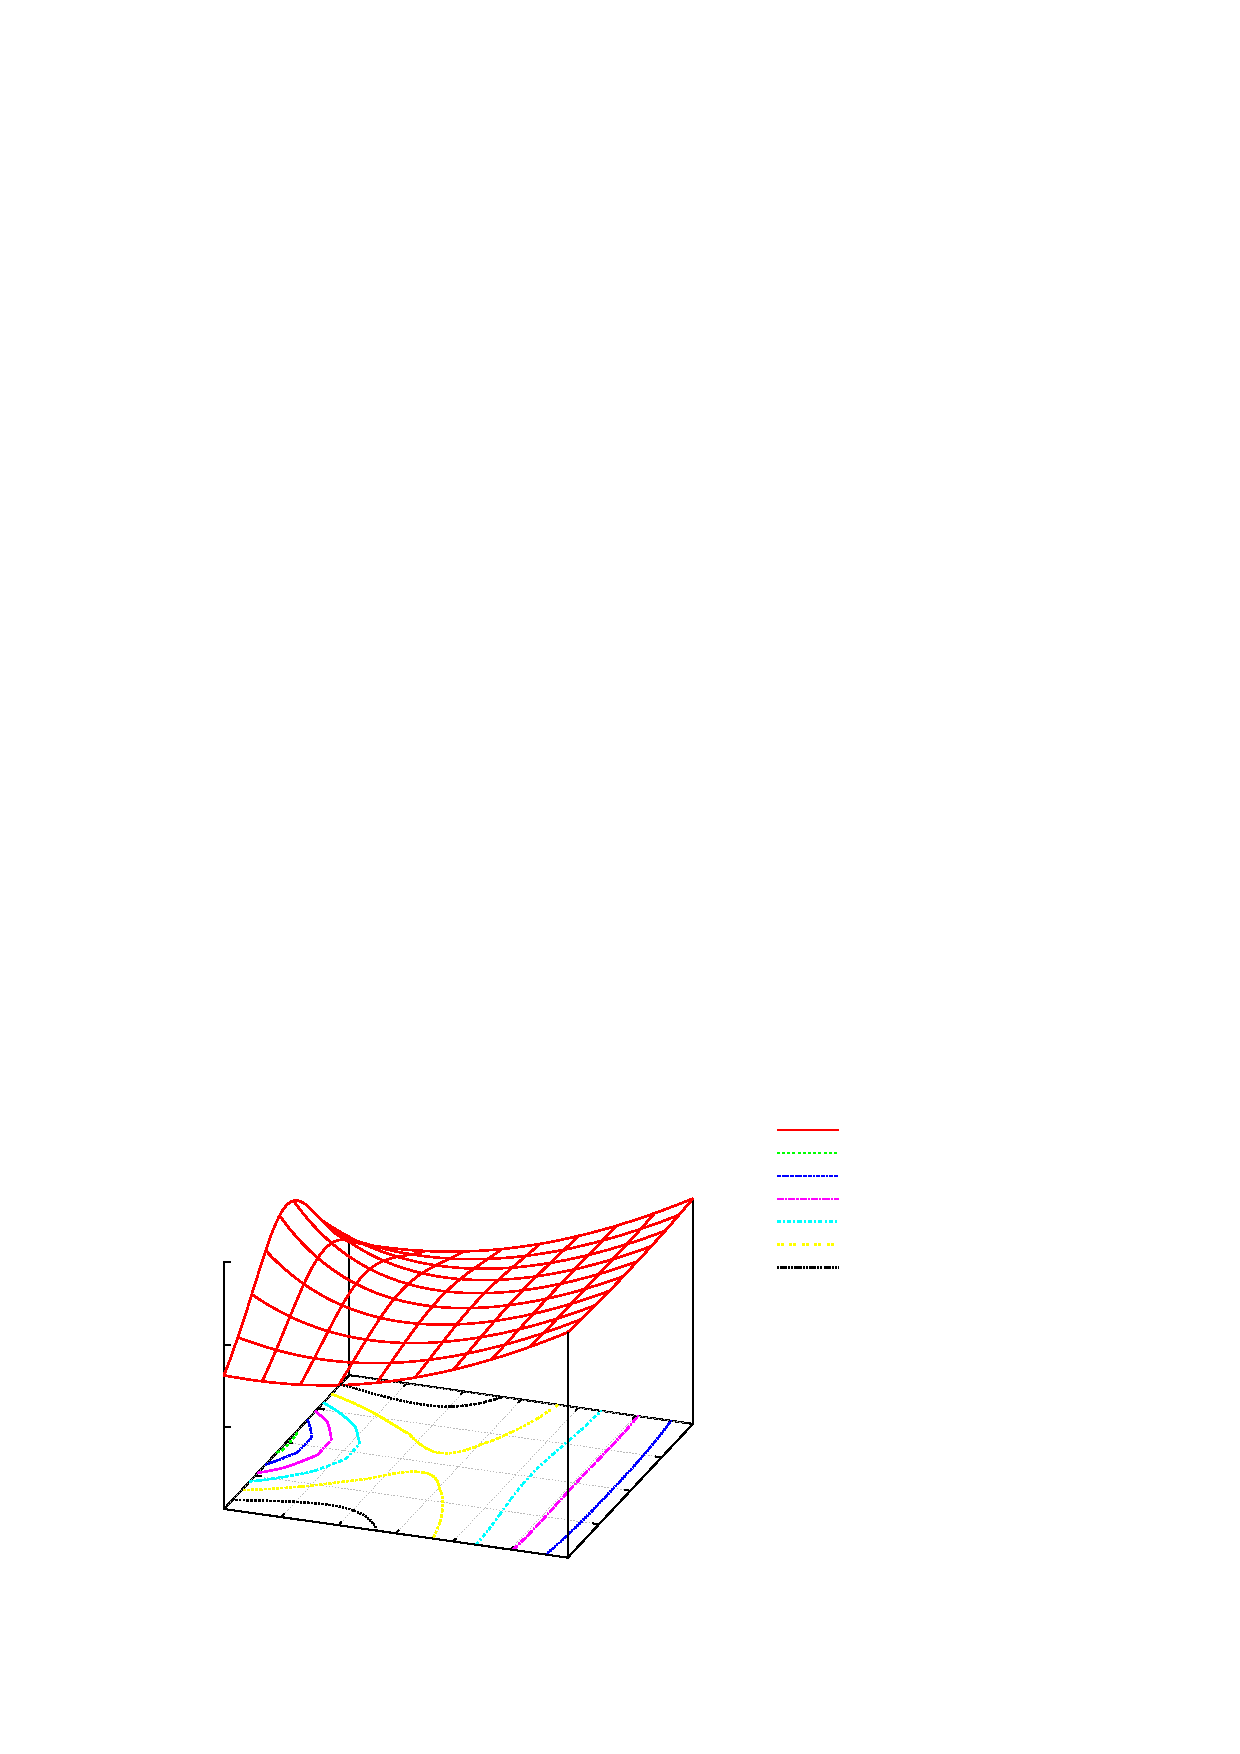
\includegraphics{Hills}}%
    \gplfronttext
  \end{picture}%
\endgroup
